\documentclass{article}

\usepackage[dblblindworkshop,final]{neurips_2026}
\workshoptitle{Agentic AI for Biological Discovery}
\usepackage{amsmath}
\usepackage{amssymb}
\usepackage{booktabs}
\usepackage{float}
\usepackage{microtype}
\usepackage{xcolor}
\usepackage{tikz}
\usetikzlibrary{arrows.meta,positioning}
\usepackage{url}
\usepackage[hidelinks]{hyperref}

\title{A Provenance-First Harness for Auditable Bayesian Clinical Trial Design}

\author{%
  Reuben N Addison, PhD \\
  DePauw University \\
  \texttt{reubenaddison@depauw.edu} \\
  \And
  Shucheng Cao \\
  McGill University \\
  \texttt{shucheng.cao@mail.mcgill.ca} \\
}

\begin{document}

\maketitle

\begin{abstract}
Clinical trial design needs a clear record of which evidence changed the prior and whether the recommendation can be reproduced. We present OpenTrial, a provenance-first harness for Bayesian design of two-arm trials. It retrieves evidence from up to eight public sources and records every source outcome. Only records with an effect estimate and standard error enter the prior; context-only records remain visible but receive no statistical weight. The numerical path is deterministic and covers random-effects pooling, power, prior-predictive assurance, Bayesian decision criteria, Monte Carlo Type I error checks, and group-sequential designs. An optional language model can summarize completed results but cannot alter any calculation.

We evaluated the offline workflow on a seeded Type 2 diabetes and HbA1c case built from four synthetic evidence records. They yielded a Normal prior with mean 0.5009 and standard deviation 0.0544. At 80 participants per arm, power was 0.885 and assurance was 0.873. A four-look O'Brien--Fleming design returned a Type I error estimate of 0.0234 against a nominal 0.025 and expected enrollment of 61.6 per arm under the alternative. Assurance fell to 0.183 under a skeptical prior, showing how strongly the recommendation depended on borrowed information. Cross-checks against SciPy and statsmodels reproduced core deterministic results to at least nine decimal places. OpenTrial is a pattern for bounded agency in clinical methods, not a validated clinical tool.
\end{abstract}

\section{Introduction}

Every clinical trial design starts with an assumed treatment effect. That choice sets sample size, cost, and participant exposure, yet its evidence is often summarized in prose or carried forward from earlier protocols. Bayesian design makes the assumption explicit as a prior, but a prior can still hide which studies were included, how duplicate reports were handled, and which records contributed numbers.

Agentic scientific systems make this problem more urgent. Language-model agents can search literature and invoke specialist tools, as shown by Coscientist, ChemCrow, and SciToolAgent \citep{boiko2023,bran2024,ding2025}. Clinical trial design is a harder accountability test than report generation. A statistician must be able to identify admitted evidence, reproduce the operating characteristics, and see whether the recommendation survives alternative priors.

OpenTrial addresses this need with a constrained harness. The user selects sources; connectors write candidate records and source outcomes to a ledger; deterministic code admits quantitative evidence, constructs a prior, and evaluates fixed and sequential designs. A language model may explain the completed analysis but cannot change it. The statistical pieces are established methods \citep{dersimonian1986,ohagan2005,obrien1979,pocock1977}. The contribution is their assembly around two enforceable boundaries: an evidence-admission rule and a one-way interface from computation to generated narrative.

\section{Related work and design principle}

Tool-using scientific agents are commonly judged by successful tool selection and task completion \citep{boiko2023,bran2024,ding2025}. Biomedical agents such as Biomni and TxAgent bring the same pattern to biology and therapeutics \citep{huang2026,gao2025}, and language models have been applied to trial tasks such as patient matching and eligibility-criteria drafting \citep{jin2024,wang2023}. To our knowledge, none builds a design prior from retrieved evidence. Trial planning adds a different requirement. Assurance averages success over prior uncertainty \citep{ohagan2005}, Bayesian practice calls for prior sensitivity \citep{spiegelhalter2004}, and repeated looks must preserve the intended false-positive rate \citep{fda2019}. These need inspectable calculations, not optional prose.

OpenTrial follows \emph{bounded agency by data type}. Retrieval can be broad, connector failures need not stop a run, and a model can explain output. Only typed quantitative records can enter the prior, however, and only tested functions can produce design metrics. The present system is therefore narrower than autonomous planning and easier to audit.

\section{System}

\subsection{Evidence ledger and admission rule}

OpenTrial supports continuous and binary two-arm endpoints. Its connectors cover ClinicalTrials.gov, PubMed, openFDA, DailyMed, Open Targets, PharmGKB, Semantic Scholar, and You.com, with a seeded offline mode for reproduction. Each connector returns a source outcome even when no usable record is found or the request fails. The report therefore distinguishes \emph{not searched}, \emph{searched with no quantitative result}, and \emph{connector error} from successful retrieval.

A candidate record contains source metadata, a study identifier where available, sample size, effect estimate \(y_i\), and standard error \(s_i\). A record affects the prior only when \(y_i\) and \(s_i>0\) are present and finite. Registry descriptions, safety counts, label text, and other context remain in the ledger but receive zero statistical weight. Multiple reports are collapsed by trial identifier when possible, then by an exact effect, standard-error, and sample-size fingerprint. The retained record and the reason for each exclusion are serialized with the analysis.

\begin{figure}[ht]
\centering
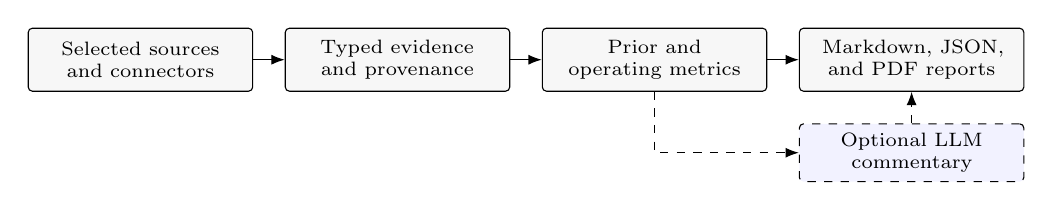
\begin{tikzpicture}[
  >=Latex,
  node distance=4mm,
  box/.style={draw, rounded corners=1.5pt, align=center, minimum height=8mm,
    text width=1.03in, font=\scriptsize, fill=gray!6},
  narr/.style={draw, dashed, rounded corners=1.5pt, align=center,
    minimum height=7mm, text width=1.03in, font=\scriptsize, fill=blue!5}
]
\node[box] (src) {Selected sources\\and connectors};
\node[box, right=of src] (ledger) {Typed evidence\\and provenance};
\node[box, right=of ledger] (stats) {Prior and\\operating metrics};
\node[box, right=of stats] (report) {Markdown, JSON,\\and PDF reports};
\node[narr, below=4mm of report] (llm) {Optional LLM\\commentary};
\draw[->] (src) -- (ledger);
\draw[->] (ledger) -- (stats);
\draw[->] (stats) -- (report);
\draw[->,dashed] (stats) |- (llm);
\draw[->,dashed] (llm) -- (report);
\end{tikzpicture}
\caption{OpenTrial's computational boundary. The dashed narrative path cannot write back to the ledger or statistical analysis.}
\label{fig:architecture}
\end{figure}

\subsection{Prior construction}

For \(k\) admitted records, the default DerSimonian--Laird calculation uses
\begin{align*}
w_i&=1/s_i^2, & \widehat{\mu}_{F}&=\frac{\sum_i w_i y_i}{\sum_i w_i},
& Q&=\sum_i w_i(y_i-\widehat{\mu}_{F})^2,\\
\widehat{\tau}^{\,2}&=\max\left\{0,\frac{Q-(k-1)}
{\sum_i w_i-\sum_i w_i^2/\sum_i w_i}\right\},
& w_i^\star&=\frac{1}{s_i^2+\widehat{\tau}^{\,2}}.
\end{align*}
The prior is \(N(\mu_0,\sigma_0^2)\), where \(\mu_0=\sum_iw_i^\star y_i/\sum_iw_i^\star\) and \(\sigma_0^2=1/\sum_iw_i^\star\). Restricted maximum likelihood is also available because heterogeneity estimates can be unstable when \(k\) is small \citep{viechtbauer2005}. The report stores the estimator, \(Q\), \(\widehat{\tau}^{\,2}\), weights, and admitted-record identifiers.

\subsection{Operating characteristics and narrative boundary}

For a continuous endpoint with common standard deviation \(\sigma\), equal allocation, and \(n\) participants per arm, \(SE_n=\sqrt{2\sigma^2/n}\). At one-sided level \(\alpha\),
\begin{align*}
\mathrm{Power}(n,\delta)&=\Phi\left(\delta/SE_n-z_{1-\alpha}\right),\\
\mathrm{Assurance}(n)&=\Phi\left(
\frac{\mu_0-z_{1-\alpha}SE_n}{\sqrt{\sigma_0^2+SE_n^2}}
\right).
\end{align*}
The engine also calculates posterior decision probabilities, predictive probability of success, prior-sensitivity scenarios, and dropout-adjusted sample sizes. Group-sequential designs use O'Brien--Fleming or Pocock boundary families and simulation-based calibration. Monte Carlo Type I checks are evaluated on draws separate from those used for calibration.

All numerical objects are complete before the optional language-model call. In the reference implementation, the model receives a serialized summary at low temperature and an instruction not to invent citations, effects, or regulatory claims. The response is stored as commentary. If the call fails, the quantitative report is unchanged and remains exportable. This makes narrative generation removable from the validation target.

\section{Evaluation}

\subsection{Seeded case and fixed design}

We used the repository's offline Type 2 diabetes case with change in HbA1c as a continuous endpoint. Its four evidence records are synthetic: they imitate registry and literature entries and describe no real trial. The assumed clinically relevant effect was \(0.5\), the endpoint standard deviation was \(1.0\), the one-sided Type I error was \(0.025\), and the target power was \(0.80\). Sample size was evaluated on a grid in increments of 20 per arm. All four records passed the admission rule (Table~\ref{tab:evidence}).

\begin{table}[H]
\caption{Synthetic seeded evidence admitted to the prior. Weights use the DerSimonian--Laird fit; \(\widehat{\tau}^{\,2}=0\) in this case.}
\label{tab:evidence}
\centering
\small
\setlength{\tabcolsep}{5.2pt}
\begin{tabular}{lrrrrr}
\toprule
Source & Year & Effect & SE & Total \(N\) & Weight \\
\midrule
ClinicalTrials.gov & 2019 & 0.48 & 0.12 & 256  & 20.6\% \\
ClinicalTrials.gov & 2020 & 0.62 & 0.15 & 188  & 13.2\% \\
PubMed             & 2021 & 0.55 & 0.10 & 1,140 & 29.6\% \\
PubMed             & 2022 & 0.43 & 0.09 & 980  & 36.6\% \\
\bottomrule
\end{tabular}
\end{table}

The records carry a nominal total of 2,564 participants. Cochran's \(Q\) was 1.52 on three degrees of freedom, so the estimated between-study variance was zero and the prior was \(N(0.5009,0.0544^2)\). Its precision was roughly equivalent to 675 participants per arm, a warning about the amount borrowed rather than a claim of exchangeability.

The continuous 80\% power crossing occurs near 63 participants per arm. With a grid step of 20, OpenTrial recommended 80, where power was 0.8854 and assurance was 0.8733. They are close because the prior is narrow and centered near the assumed effect.

\subsection{Sequential design and prior sensitivity}

A four-look O'Brien--Fleming design evaluated information fractions of 0.25, 0.50, 0.75, and 1.00, corresponding to 20, 40, 60, and 80 participants per arm. Table~\ref{tab:sequential} reports the calibrated efficacy boundaries and cumulative stopping probabilities under the alternative.

\begin{table}[H]
\caption{Four-look group-sequential design. The final column is the probability of having crossed an efficacy boundary by that look under the alternative.}
\label{tab:sequential}
\centering
\small
\setlength{\tabcolsep}{8pt}
\begin{tabular}{rrrrr}
\toprule
Look & Information & \(N\)/arm & Boundary \(Z\) & Cumulative stop \\
\midrule
1 & 0.25 & 20 & 4.08 & 0.006 \\
2 & 0.50 & 40 & 2.89 & 0.260 \\
3 & 0.75 & 60 & 2.36 & 0.654 \\
4 & 1.00 & 80 & 2.04 & 0.877 \\
\bottomrule
\end{tabular}
\end{table}

The separate null simulation returned a Type I error estimate of 0.0234 against the nominal 0.025. Expected enrollment under the alternative was 61.6 per arm, 23\% below the fixed maximum, with power 0.877 against 0.885 for the fixed design. The report does not retain Monte Carlo confidence intervals, so the Type I value is a diagnostic, not proof of exact control.

The skeptical and enthusiastic priors are \(N(0,s^2)\) and \(N(\delta,s^2)\) with \(s=\delta/z_{0.95}=0.304\) \citep{spiegelhalter2004}; the reference prior is \(N(0,1)\). At \(n=80\), assurance was 0.873 under the evidence-derived prior, 0.710 under the enthusiastic scenario, 0.380 under the reference scenario, and 0.183 under the skeptical scenario. Skeptical predictive probability of success was 0.154. The design therefore looked strong only with substantial historical borrowing, a dependence that power at \(\delta=0.5\) did not expose.

\subsection{Numerical checks}

The offline regression suite contains 133 tests and requires no network access or keys. Independent SciPy and statsmodels paths, closed forms, and numerical integration reproduced deterministic prior, power, assurance, and meta-analysis results to at least nine decimal places. These checks are separate from the renderer and narrative model.

Validation exposed a circular Type I check that reused calibration paths and could return the target by construction. Evaluation now uses separate draws. It also exposed a heterogeneity term that double-counted sampling error. Both errors had produced plausible summaries.

\section{Discussion}

OpenTrial's main result is not the automation of standard formulas. It is the assignment of different trust levels to retrieval, statistical admission, calculation, and explanation. A connector may return useful context without a usable effect, and a model may clarify a report without choosing the prior. Every weighted datum has provenance, every exclusion has a reason, and headline numbers exist before narrative generation.

The current system is not an autonomous trial designer. Source selection is user-guided, and the optional model neither plans tool calls nor changes the analysis. Future versions could propose searches, but that autonomy should be judged by evidence recall, duplicate detection, extraction accuracy, and design stability rather than report fluency.

\subsection{Limitations and intended use}

One synthetic seeded case cannot measure live-source coverage, extraction accuracy, connector drift, or contradictory literatures. Numeric fingerprinting may miss related publications or collapse distinct records with identical summaries. With four studies, \(\widehat{\tau}^{\,2}\) is weakly identified, and zero does not establish homogeneity.

The continuous calculation assumes a Normal endpoint, equal allocation, and known standard deviation. The prototype lacks covariate adjustment, multiplicity, estimand changes, and missing-data models beyond dropout inflation. We have not run a prospective comparison with trial statisticians or a formal narrative-faithfulness study.

OpenTrial is a methods prototype, not a validated clinical tool. Enrollment, stopping rules, and regulatory strategy require independent statistical review. Broader benchmarks remain necessary.

\clearpage
\bibliographystyle{plainnat}
\bibliography{references}

\end{document}
